\documentclass[a4paper]{article}
\usepackage{amsmath}
\usepackage{amsfonts}
\usepackage{amssymb}
\usepackage{graphicx}
\usepackage{hyperref}
\usepackage{listings}
\usepackage[left=2cm,right=2cm,top=2cm,bottom=2cm]{geometry}
\begin{document}
\title{Reveal.js Tutorial}
\author{by Kostas and Craig}
\maketitle

In this tutorial we will create a presentation by constructing everything from scratch: HTML, CSS, Markdown and JavaScript.
Before we start the tutorial it is useful to have a quickly go through the main elements of web-page building.

\section{Crash-course}
These \textit{cheat-sheets} have been built from resources available on \emph{CodeAcademy} and the \emph{Mozilla Developer Network} which are also recommended for more in-depth training and resources. An excellent online book is also available on \url{http://eloquentjavascript.net/}.

We decided that the quickest way to approach this is to provide commented samples so we can quickly build a simple web-page.

\subsection{HTML}
HTML (\emph{HyperText Markup Language} is used by browsers to communicate with each other and display data in an attractive fashion. It has a tree-like structure similar to that of XML. Each branch defines a section of a web page is started by some text in brackets \texttt{<branch>} and ends with a \textbf{backward} slash and the text \verb|<\branch>|. Some objects are added in self-stopping branches by using a \textbf{forward} slash before closing the bracket \texttt{<branch/>}
\begin{table}

\noindent\begin{tabular}{l l}

\begin{lstlisting}[language=HTML]
<!doctype html>
<html>
\end{lstlisting}
  & \parbox{0.4\textwidth}{Both do the same thing. Only the first is necessary in HTML v$\geqslant 4$}\\[2ex]
\begin{lstlisting}[language=HTML]
<head>
	<title>Amazed</title>|
	<link rel="stylesheet" type="text/css"
		 href="coolStyle.css"/>
</head>
\end{lstlisting}
 &\parbox{0.4\textwidth}{The branch specifies information that is first read by the browser to correctly display the page. This is where JavaScript source files and CSS files are conventionally specified. It also contains other branches such as tags/titles/authors/etc used by search engines}\\
\begin{lstlisting}[language=HTML]
<body>
\end{lstlisting}
 &\parbox[t]{0.4\textwidth}{This is the part where the data goes that is displayed	to the user.}\\[2ex]
\quad\verb|	<h1>Amazing Presentations Ltd.</h1>|& Display text using heading 1\\[2ex]
\quad\verb|	<div class="wow">|& \\[2ex]
\qquad\verb|		<h2>Amazing discovery.</h2>|&\\[2ex]
\qquad\verb|		<p>Something that changes the world.</p>|\ref{p}&\\[2ex]
\qquad\verb|		<a href="otherPageLoc.html">Lookie here.</a>|&\\[2ex]
\quad\verb|	</div>|&\\[2ex]
\quad\verb|	<p id = "footer">&copy;NGCM Ltd.</p>|&\\[2ex]
\verb|</body>|&\\[2ex]

\end{tabular}
\end{table}

\subsection{CSS}
CSS or Cascading Style Sheets are commonly used in web applications to standardise formatting and styles. It is also used in reveal.js to set-up a presentation template.


\begin{tabular}{l l}

\begin{lstlisting}[language=HTML, label=body]
body {
	height: 100%;
	margin: 0;
	text-align: center;
	width: 100%;
}
\end{lstlisting} & Specifies the general layout of the page.\\
\begin{lstlisting}[language=HTML, label=p]
p {
	font-size: 2rem;
}
\end{lstlisting} & Set the font size of text inside \verb|<p></p>|\\
\begin{lstlisting}[language=HTML, label=wow]
.wow {
  font-family: Helvetica, sans-serif;
  background-image: url("cool.jpg");
  background-size: cover;
  color: #ffffff
}
\end{lstlisting} & \parbox{0.4\textwidth}{Specify properties of a page division, i.e. a \texttt{<div>} part of a page that should have special properties (e.g. a background image)}\\
\begin{lstlisting}[language=HTML, label=wowA]
.wow a {
	color: #00FFAA;
	text-decoration: none;
	font-size: 1.25em;
}
\end{lstlisting} & \parbox{0.4\textwidth}{Inside a division it might be necessary to want to change the way a link is formatted (the \texttt{<a>} inside a \texttt{<div>}.}\\
\begin{lstlisting}[language=HTML, label=footer]
#footer{
  font-size:0.75rem;
}
\end{lstlisting} & \parbox{0.4\textwidth}{If a specific paragraph's has to be formatted differently (e.g. change only the colour) you can give it an ID and set it up here.}\\

\end{tabular}

\subsection{JavaScript}
HTML contains static content and JavaScript is the way by which a web-page becomes dynamic. This is a scripting language that is interpreted by your browser and it is able to do what most programming languages do: mathematical operations, run loops, functions and create objects.

\small{JavaScript is completely different from Java}
\subsection{Markdown}
Markdown is very useful for writing content for web-pages books and other types of documents. The language is similar to \LaTeX in the sense that it uses plain text to write the source for a nicely formatted document, but it has the advantage of having very human-readable source code. The best way to write markdown is to use a specialised editor such as Atom, but in this tutorial we will use Brackets with a plugin for MD live generation. Markdown is so simple that an actual tutorial is not required for the basics and the cheat-sheet below should prove sufficient (for a step-by-step 10 minute tutorial check \url{http://commonmark.org/help/tutorial/} ):
\begin{figure}[!HT]
\centering
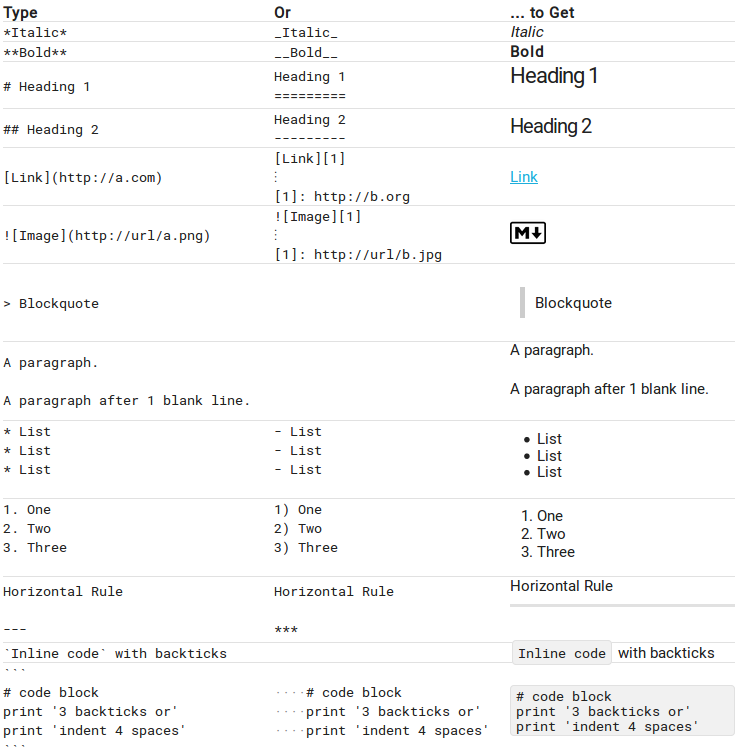
\includegraphics[scale=0.6]{MD-Tutorial.png}
\end{figure}

\section{Tutorial}
The tutorial exercise is to create a presentation by yourself from the bottom-up.
\footnote{The above structure does not have to be necessarily respected, but it is recommended for cross-compatibility among browsers and connection speed (this unlikely to be a problem), since HTML is normally loaded progressively, it is necessary to have all the elements required for the next processing steps)}
\begin{itemize}
\item Start with the basic HTML structure, i.e. the \texttt{<html>} tags with \texttt{<head>}, \texttt{<body>}, etc.
\item Add the reveal.js stylesheet and your own in the <head> branch.
\item Add the \textit{reveal} \texttt{<div>} and inside it the \textit{slides} \texttt{<div>}
\item Add about five sections inside the slides \texttt{<div>}
\item Create \underline{two} JavaScript sections to call \textit{reveal.js} and \textit{head.min.js} (this is needed so that it works in all browsers),found in \texttt{./reveal.js/js/} and \texttt{./reveal.js/lib/js/}, respectively.
\item After the slides section a new script branch is added to initialise the presentation.
\end{itemize}
\end{document}
